\documentclass{standalone}
\begin{document}
	\subsection{Kernel Size Optimization}
	
	During the building of the multi channel image, we have to compute different image features, that requires the setting of different parameters.
	To properly set these parameters I've build a routine to estimate the best values.\\
	To build this routine I've used the tools given by scikit-optimize library. The idea behind the optimization process is very simple but requires some ground truth labels. I've simply generates many set of parameters, train the centroids with this set and label some images, after that I've compute the according of this labels with ground truth ones. After that I've simply chose the set of paramenter which guarantees the best according with the references. The whole procedure is schetced is \figurename\,\ref{ref:ParamOpt}
	
	\begin{figure}
		\centering
			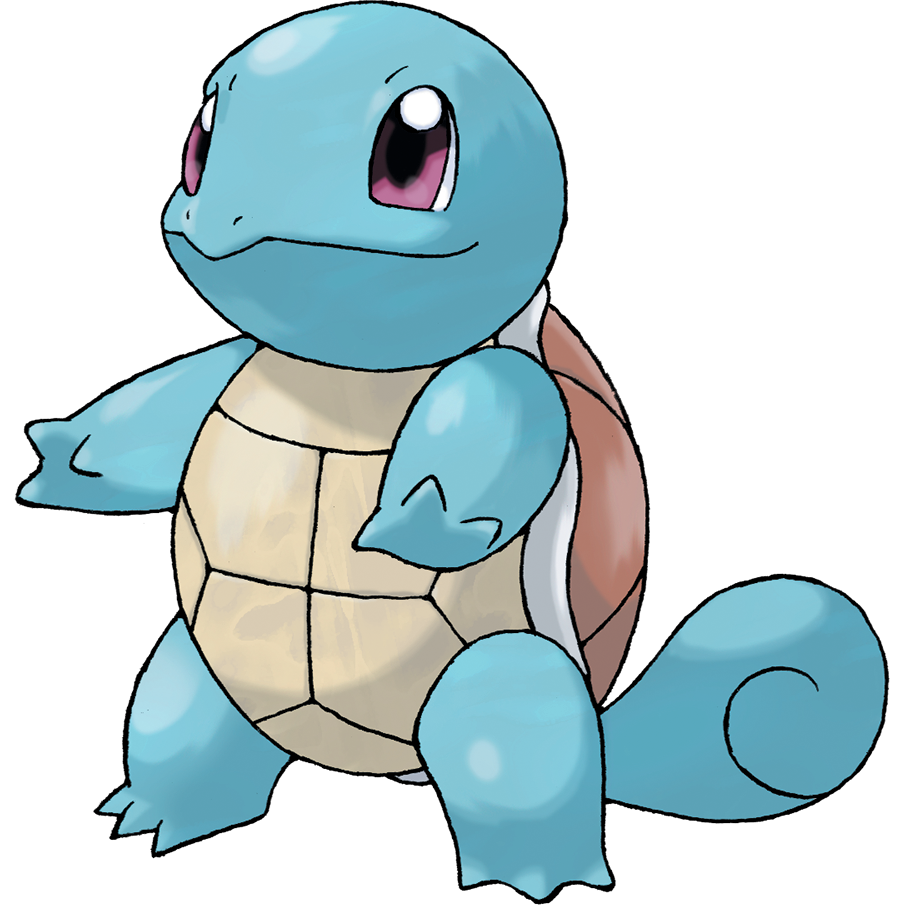
\includegraphics[scale=.1]{PlaceHolder.png}
			\label{fig:ParamOpt}\caption{} 
	\end{figure}

	This process allows to optimize the parameters in order to obtain the best results as possible. As reference labels I've used the one provided by the public datasets ZENODO and MOSMED. This optimization allows to achieve a better segmentation, but isn't necessary and doesn't interfere to the actual centroids estimation, keeping the techniques unsupervised.
\end{document}